%!TEX root = ./main.tex

% content goes here 
    
    \section{Git}
	\begin{frame}
		\frametitle{Git}
		% \framesubtitle{}
		\begin{columns}[c]
    		\column{.5\textwidth} 
        		\begin{itemize}
					\item Collaborate
                    \item Version Control
                    \item Open Source
          		\end{itemize}
          	\column{.5\textwidth}
            	\centering
				
\includegraphics[width=.7\linewidth,]{res/git}

				\vspace{1cm} % blank lines around this are needed

				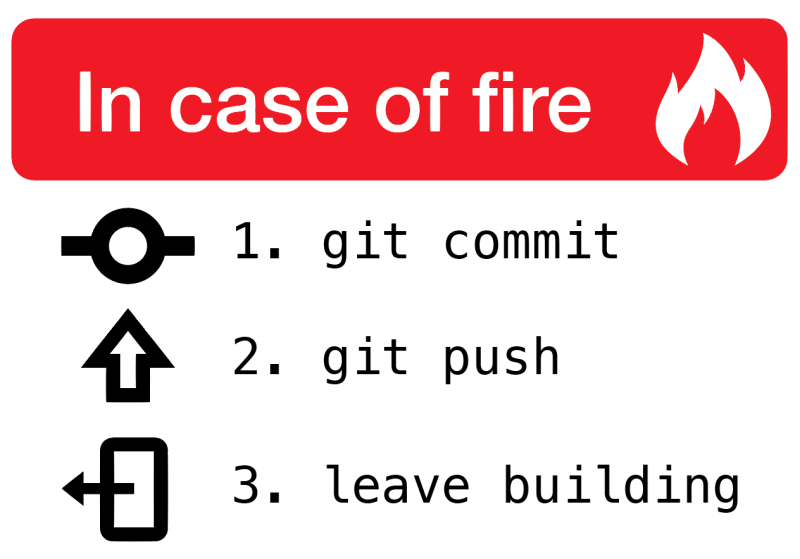
\includegraphics[width=.7\linewidth]{res/fire}
        \end{columns}
	\end{frame}
    
    \subsection{Workflow}
    \begin{frame}[allowframebreaks=10] % "=10" -> do not auto frame break
		\frametitle{Workflow}
		% \framesubtitle{}
        \begin{figure}
        	\centering
        	\includegraphics[width=0.8\linewidth]{"res/git_client-server"} \\
        \end{figure}
	\end{frame}
	
	
	
	\section{Account}
    \begin{frame} 
		\frametitle{Create a git account}
		\link{https://github.com/}{github.com}
		\begin{itemize}
			\item Gebruik studentenmail: voornaam.achternaam@student.uantwerpen.be
			\item Gebruik herkenbare naam
		\end{itemize}

		\link{https://education.github.com/}{Student developer pack}
		\begin{itemize}
			\item \textbf{Geeft mogelijkheid tot private repositories!}
		\end{itemize}
		
	\end{frame}
	
	\section{PyCharm}
    \begin{frame} 
		\frametitle{Git in PyCharm}
		 \begin{enumerate}
		 	\item Type: $Ctrl+Alt+s$
		 	\item Navigeer naar: $Version\: Control - GitHub$
		 	\item Add account
		 \end{enumerate}
	\end{frame}
	
	\section{Gitignore}
    \begin{frame}
		\frametitle{.gitignore}
		% \framesubtitle{}
        \begin{enumerate}
        	\item Maak .gitignore file in root van project
        	\item Best toe te voegen (voor nu)
        	\begin{itemize}
        		\item $.idea$
        		\item $\_\_pycache\_\_$
        		\item $venv$
        		\item $env$
        	\end{itemize}
        	\item Ook regex mogelijk (*.txt)
        \end{enumerate}
	\end{frame}
		
	\section{Nieuw project}
    \begin{frame} 
		\frametitle{Instellingen bij een nieuw project}
		\begin{enumerate}
			\item Nieuwe github repository
				\begin{itemize}
					\item Zet type op \textbf{Private}!
				\end{itemize}
			\item Check out from Version Control - Git
			\item Kies project uit dropdown of plak URL		
		\end{enumerate}
	\end{frame}
	
	\section{Bestaand project}
	\begin{frame} 
		\frametitle{Beginnende van een bestaand project}
		\begin{enumerate}
			\item VCS
			\item Import into Version Control - Create git repository
			\item Import into Version Control - Share project on GitHub
			\item Laat best naam staan
			\item Zet op private (Remote: origin niet aanpassen)		
		\end{enumerate}
	\end{frame}
		
    \section{Basics}
    \begin{frame} 
		\frametitle{Basics}
		\begin{itemize}
			\item commit
			\item push
			\item pull
		\end{itemize}
	\end{frame}
	
	\section{Don'ts}
    \begin{frame} 
		\frametitle{Don'ts}
		\begin{itemize}
			\item Niet werkende code pushen
			\item Push nooit code die afhankelijk is van absolute paden
			\item Push geen persoonlijke folders (pycache, env) $\rightarrow$ .gitignore
		\end{itemize}
	\end{frame}
	
	\section{Do's}
    \begin{frame} 
		\frametitle{Do's}
		\begin{itemize}
			\item \textbf{Pull voordat je een push doet}
		\end{itemize}
	\end{frame}
	
	\section{Merge conflicts}
	\begin{frame}
		\frametitle{Merge conflicts I}
		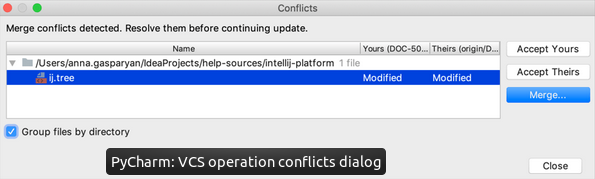
\includegraphics[scale=0.5]{res/mergeconflict1.png}
		
		
	\end{frame}
	\begin{frame}
		\frametitle{Merge conflicts II}
		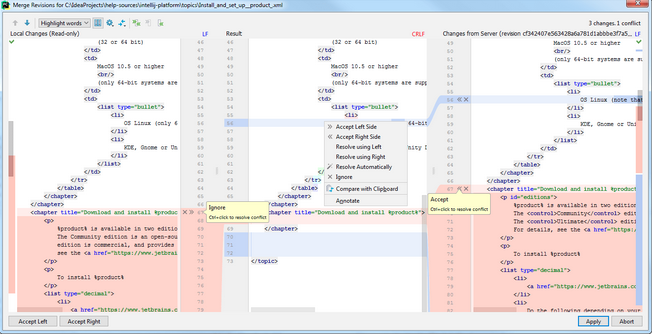
\includegraphics[scale=0.45]{res/mergeconflict2.png}
	\end{frame}
	
	
	
	

	% end of content
